Before discussing the specifics of the model selection process, some terminology should be discussed. The \textit{batch} used in training is the number of inputs that are used for a single prediction. For example, with a batch size of 31, the network is using the past month of information to predict the $32^{nd}$ day's information. When discussing an \textit{LSTM layer with n nodes}, this is in reference to \textit{n} of the nodes depicted in Figure \ref{fig:MemoryCells}, where each node takes information from the entire batch. \textit{Activation functions} were discussed previously in Section \ref{sec:intro}, but the main idea is that they are functions that restrain the range of values, mapping each input to a corresponding output. A \textit{dropout layer} is not so much a layer in the physical sense, but is rather a method of regularization applied to the previous layer. For example, a dropout layer with a rate of 5\% means that in each training iteration, there is a 5\% chance of any node being turned off. This process helps avoid over\-fitting, which is a common issue with deep learning models.

To create the LSTM network, the \textit{Keras} framework within Python was used \citep{chollet2015keras}. There are several powerful tools for building machine learning models, but \textit{Keras} was chosen because of the ease of use and ability to take advantage of hyperparameter tuning when optimizing the model. The initial steps of model creation involved imputation (discussed in Section \ref{sec:EVER}), creating a simple model that could be made more complex over time, and splitting the data into a testing and training set. The training set was chosen to be the first 90\% of the data between 1995 and 2023, leaving the remaining 10\% for testing. The initial model contained a single LSTM layer with 128 nodes, each of which used the ReLU activation function for the `Candidate Output' and `Candidate Cell State Addition' in Figure \ref{fig:MemoryCells}. Note that the gates used the sigmoid activation function, which is the default in \textit{Keras}. Once the initial model was trained, code was adapted from \cite{lstmkeras} to get out-of-sample predictions. All code is available on \href{https://github.com/lliucci/Writing-Project}{GitHub}.

Once a base framework and method for validation was created, the structure of the model could be tweaked. This was done by implementing a random search across a set parameter space. The base model contained 3 LSTM layers and 3 Dropout layers. Parameters that were defined to be searched within each LSTM layer were the number of nodes (minimum of 8 with a maximum of 64) and the activation function (either ReLU or Tanh). For the Dropout layers, the dropout rate was chosen to be either 1\%, 5\%, 10\%, or 15\%. Fixed parameters include the kernel regularizer (L1 norm with a rate of 0.001) and the activity regularizer (L2 norm with a rate of 0.001).

The random search comprised of 50 randomly chosen combinations that were trained for 30 iterations each. The best model was chosen as the model with the lowest mean squared error when compared to the testing data set. The best model had the following structure;

\begin{itemize}
    \item LSTM Layer: 17 Nodes, ReLU Activation
    \item Dropout Layer: Rate of 15\%
    \item LSTM Layer: 11 Nodes, Tanh Activation
    \item Dropout Layer: Rate of 15\%
    \item LSTM Layer: 37 Nodes, Tanh Activation
    \item Dropout Layer: Rate of 5\%
\end{itemize}

This model was trained for an additional 20,500 iterations. A figure containing the training progress is shown in Figure \ref{fig:Training}. A key idea to note from the training process is that after about 12,000 iterations, the model performance becomes fairly constant with only minor improvements over time.

\begin{figure}[ht]
    \subfloat[2,530]{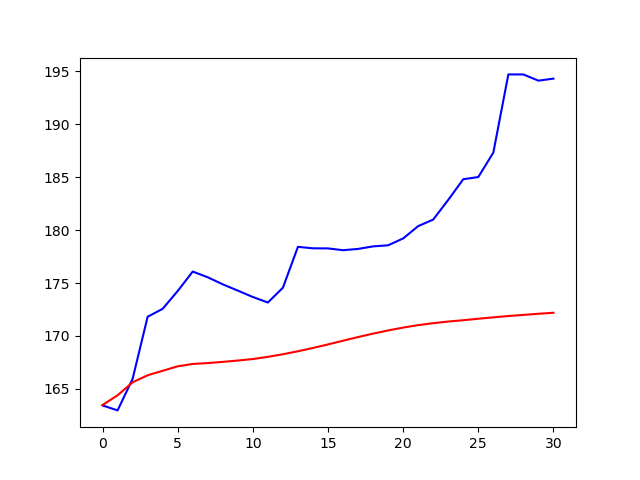
\includegraphics[width = 0.2\linewidth]{"../../Model Diagnostics/model_0.png"}}
    \subfloat[4,530]{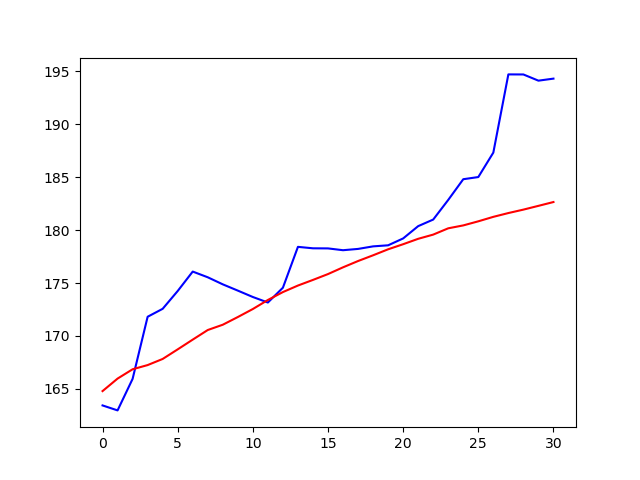
\includegraphics[width = 0.2\linewidth]{"../../Model Diagnostics/model_1.png"}}
    \subfloat[6,530]{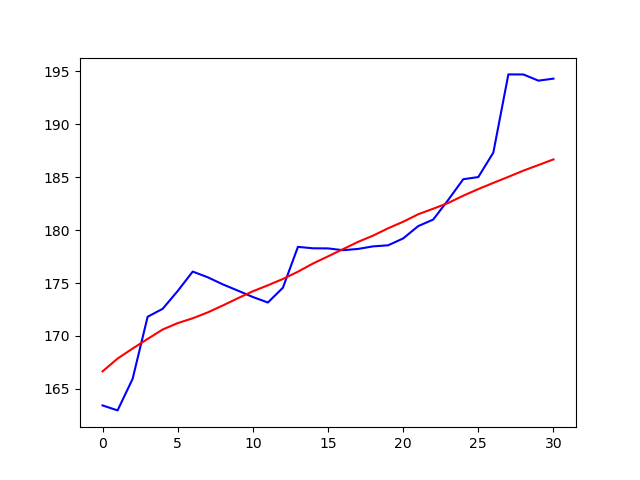
\includegraphics[width = 0.2\linewidth]{"../../Model Diagnostics/model_2.png"}}
    \subfloat[8,530]{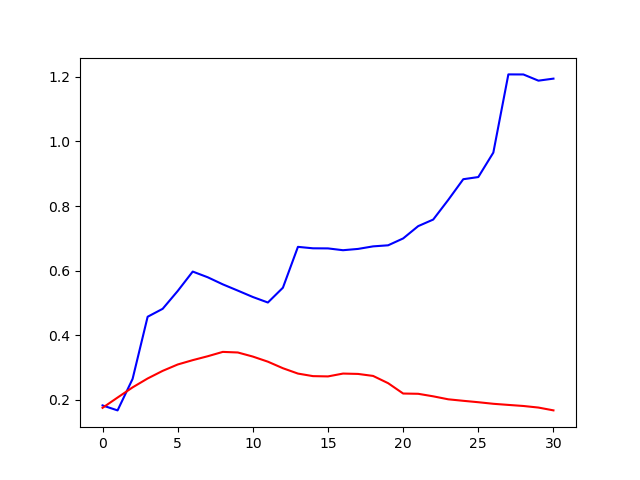
\includegraphics[width = 0.2\linewidth]{"../../Model Diagnostics/model_3.png"}}
    \subfloat[10,530]{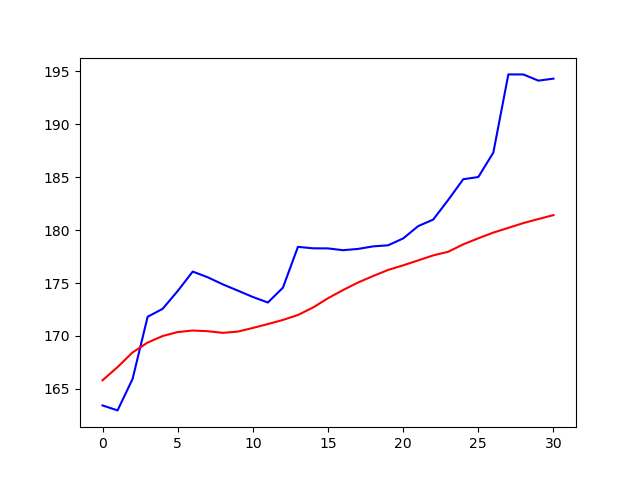
\includegraphics[width = 0.2\linewidth]{"../../Model Diagnostics/model_4.png"}}\\
    \subfloat[12,530]{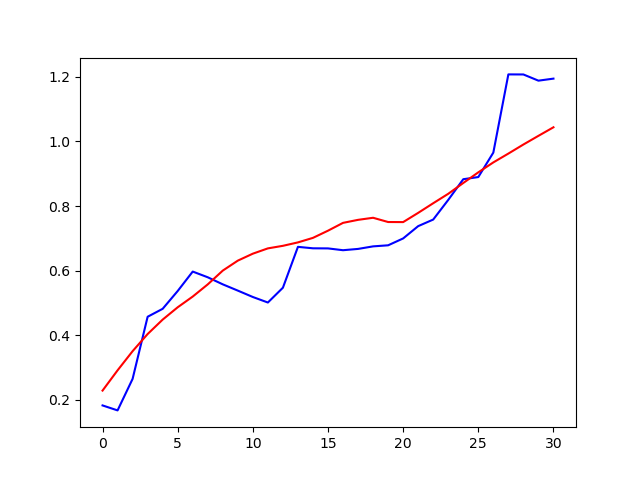
\includegraphics[width = 0.2\linewidth]{"../../Model Diagnostics/model_5.png"}}
    \subfloat[14,530]{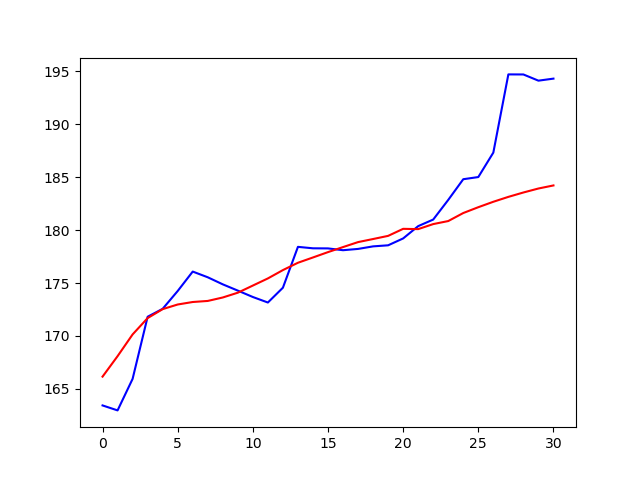
\includegraphics[width = 0.2\linewidth]{"../../Model Diagnostics/model_6.png"}}
    \subfloat[16,530]{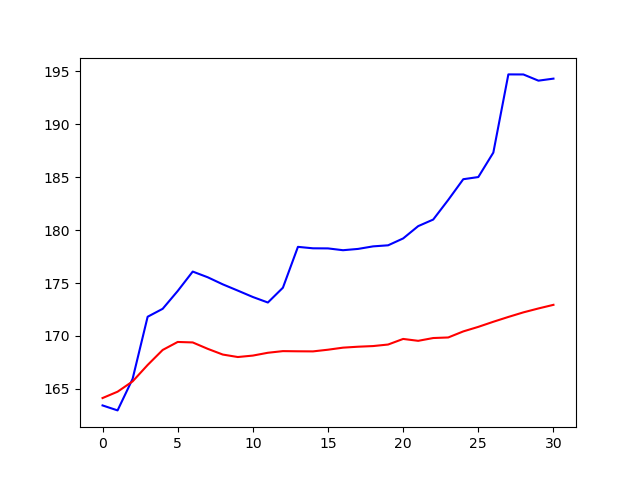
\includegraphics[width = 0.2\linewidth]{"../../Model Diagnostics/model_7.png"}}
    \subfloat[18,530]{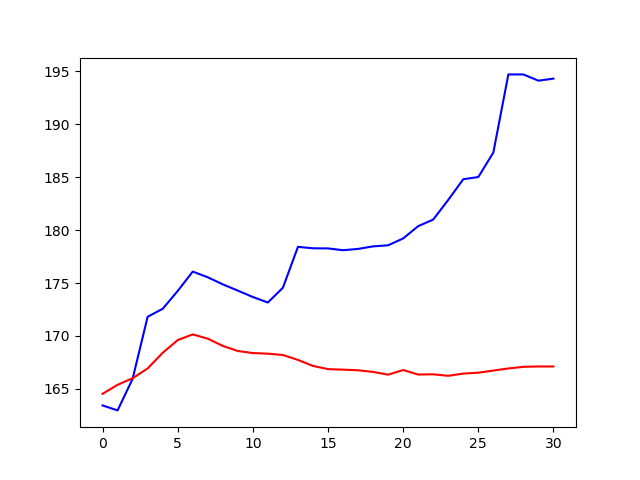
\includegraphics[width = 0.2\linewidth]{"../../Model Diagnostics/model_8.png"}}
    \subfloat[20,5530]{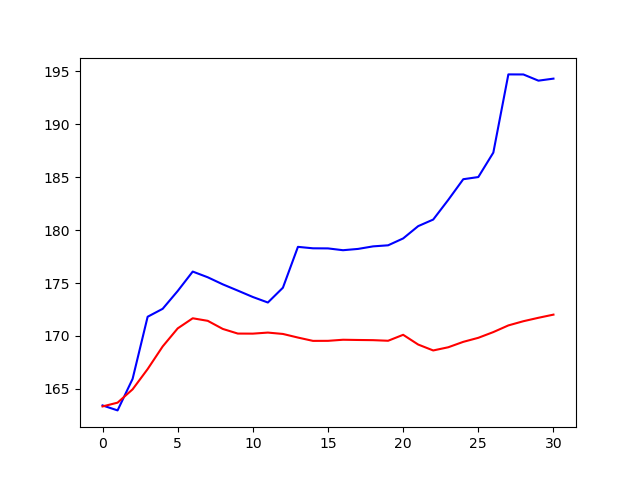
\includegraphics[width = 0.2\linewidth]{"../../Model Diagnostics/model_9.png"}}
    \caption{A series of plots obtained from the training process. Each plot shows the predicted water depths 31 days past the training set. The red line indicates the predictions from the LSTM and the blue line indicates the observed water depth. The number below each plot indicates how many generations the LSTM was trained for when the predictions were made.}
    \label{fig:Training}
\end{figure}

In order to get a sense of the variability that can arise in the training process, 5 models were initialized with the same structure (determined by the random search of hyperparameters). These 5 models were all trained on the same training data and evaluated on the same testing data. Comparisons of forecasts to the observed time series are shown in Figure \ref{fig:Variability}. Looking at plot a), it can be seen that the 5 models perform similarly after 2,000 iterations of training. After 4,000 iterations, the 5 models start to break up as they all find different weights and biases in the training process. After 6,000 iterations, model 2 outperforms all other models in the first 10 days of forecasting. After 8,000 iterations, model 2 continues to improve while models 3 and 5 gain considerable improvement. At 10,000 iterations, models 2, 3, and 5 are by far the best performing models in the 31 day forecast while models 1 and 4 struggle to correctly predict after 3 days. 

This graphic is not a perfect measure of variability in predictions as each model contains different weights and biases despite having the same structure. The purpose of these graphics is to show how the LSTMs can vary when given the same training data, same structure, and same training time. If validation data were not available, it would be difficult to trust the model's predictions as some perform great while others fall short. 

\begin{figure}[ht]
    \centering
    \subfloat[2,000]{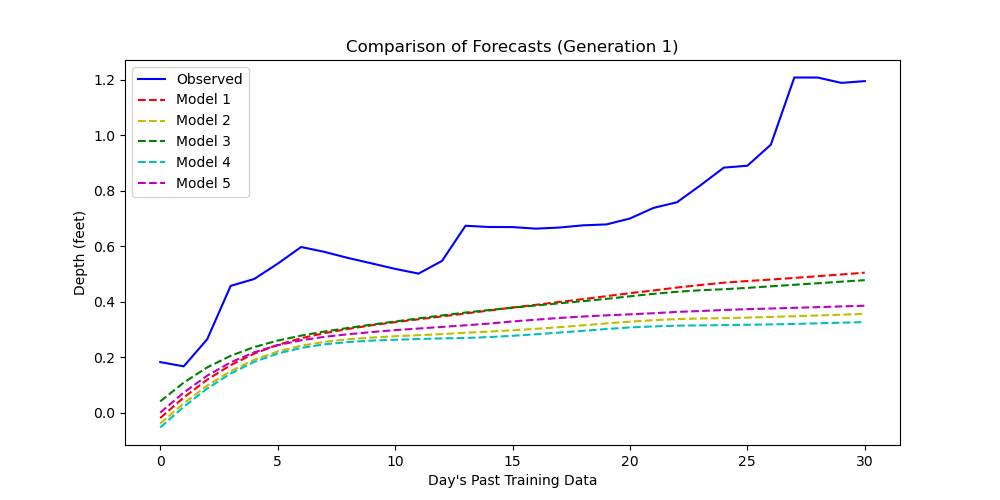
\includegraphics[width=0.5\linewidth]{"Figures/Variability_2000_Epochs.png"}}
    \subfloat[4,000]{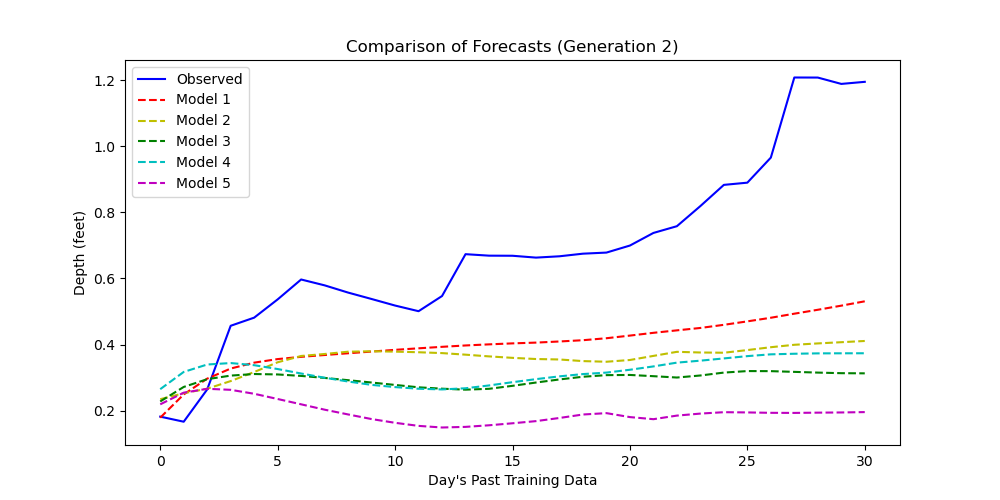
\includegraphics[width=0.5\linewidth]{"Figures/Variability_4000_Epochs.png"}}\\
    \subfloat[6,000]{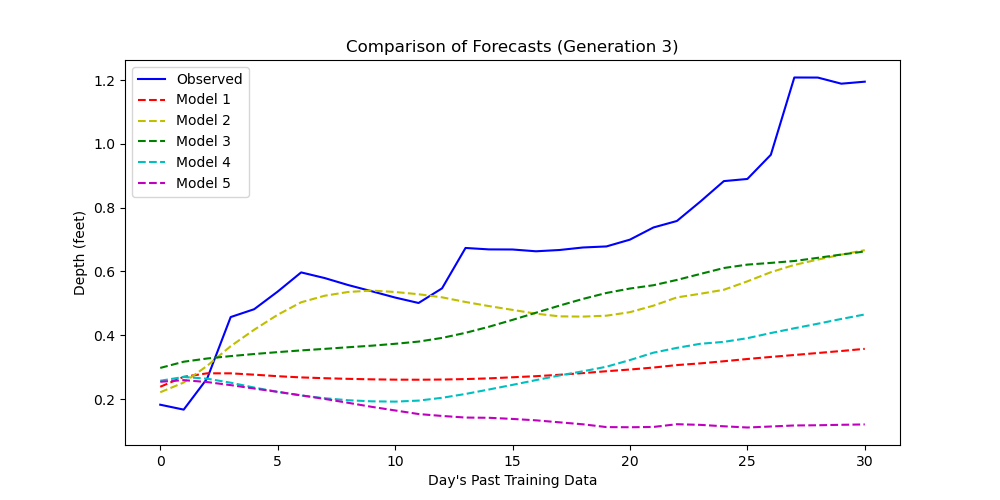
\includegraphics[width = 0.5\linewidth]{"Figures/Variability_6000_Epochs.png"}}
    \subfloat[8,000]{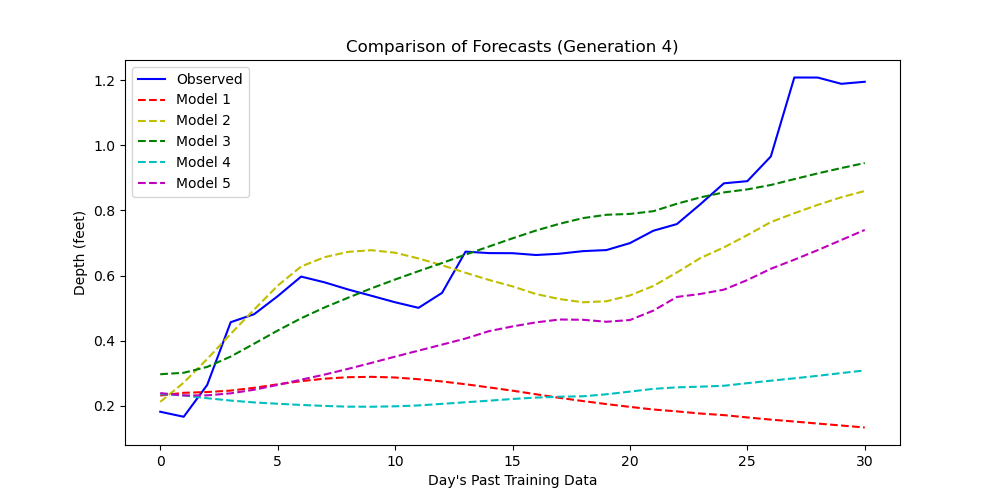
\includegraphics[width = 0.5\linewidth]{"Figures/Variability_8000_Epochs.png"}}\\
    \subfloat[10,000]{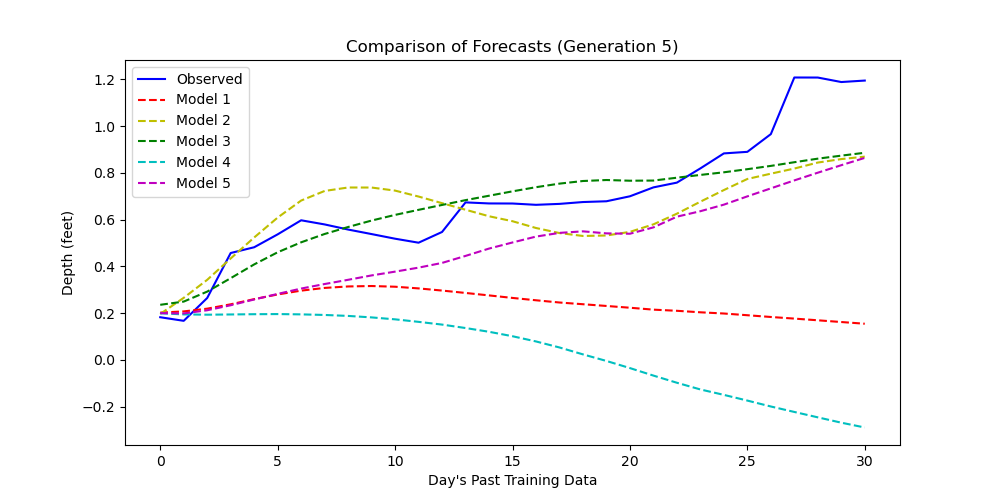
\includegraphics[width=0.5\linewidth]{"Figures/Variability_10000_Epochs.png"}}
    \caption{A line plot comparing the 1 month out-of-sample predictions for 5 models initialized with the same framework. Each model was trained on the same training data for the number of iterations displayed below the plot.}
    \label{fig:Variability}
\end{figure}

\clearpage